% !TEX root =  ../../thesis.tex

\chapter{Bayesian linear mixed effects model}
\label{ch : blmm}

\section{Introduction to linear mixed model}
\label{sec : lmm}
A linear mixed effects model, also known as linear mixed model(LMM) is a statistical model for data which is hierarchical in structure. For e.g. one such hierarchy could be, repeated observations taken from multiple patients and patients grouped under multiple hospitals. The specialty of these models is that apart from the fixed effects, they also model the correlation between the observations falling in the same group at a certain level in the hierarchy. The correlation is modeled using the random effects and the response is modeled as a linear function of both fixed and random effects.\\

There are many synonymous terminologies for data sets which are hierarchical in nature albeit with subtle nuances differentiating them. In this thesis our focus will be on Longitudinal data sets. A longitudinal data set is the one where multiple observations are collected from subjects at different points in time. For e.g. measurement of Hemoglobin of 20 patients with observations taken every month for a period of 24 months. The observations collected from a subject will be correlated, and given the fact that a linear model imposes homoscedasticity, it is not suitable for use in such scenarios.

\subsection{LMM definition}
\label{subsec : lmm_definition}
Following the notations from \citet{lesaffre_bayesian_2012}, the LMM for the observations of the $i^\text{th}$ subject among the $n$ subjects is given by

\begin{equation}
\label{eq : lmm_definition}
\boldsymbol{y}_i = \boldsymbol{X}_{i}\boldsymbol{\beta} + \boldsymbol{Z}_{i}\boldsymbol{b}_{i} + \boldsymbol{\varepsilon}_{i}
\end{equation}

where $1 \le i \le n$,\\
$\boldsymbol{y}_i = {(y_{i1}, y_{i2}, \ldots, y_{im_i})}^T$ is a vector of observations for the $i^\text{th}$ subject taken at $m_i$ time points,\\
$\boldsymbol{X}_i = {(\boldsymbol{x}_{i1}^T, \boldsymbol{x}_{i2}^T, \ldots, \boldsymbol{x}_{im_i}^T)}^T$ is the $m_i \times (d+1)$ design matrix for the $i^\text{th}$ subject,\\
$\boldsymbol{\beta} = {(\beta_0, \beta_1, \ldots, \beta_d)}^T$ is a $(d+1) \times 1$ vector of fixed effects with $\beta_0$ being the intercept,\\
$\boldsymbol{Z}_i = {(\boldsymbol{z}_{i1}^T, \boldsymbol{z}_{i2}^T, \ldots, \boldsymbol{z}_{im_i}^T)}^T$ is the $m_i \times q$ design matrix of covariates multiplying the random effects,\\
$\boldsymbol{b}_i = {(b_{0i}, b_{1i}, \ldots, b_{(q-1)i})}^T$ is a $q \times 1$ vector of random effects with $b_{0i}$ being the random intercept. The random effects $\boldsymbol{b}_i \sim N_q(\boldsymbol{0}, G)$ with $G$ being the $q \times q$ covariance matrix,\\ 
$\boldsymbol{\varepsilon}_{i} = {(\varepsilon_{i1}, \varepsilon_{i2}, \ldots, \varepsilon_{im_i})}^T$ is a $m_i \times 1$ vector of measurement errors. The errors $\boldsymbol{\varepsilon}_{i} \sim N_{m_i}(\boldsymbol{0}, R_i)$ with $R_i$ being the $(m_i \times m_i)$ covariance matrix of errors,\\

The errors $\boldsymbol{\varepsilon}_{i}$ and the random effects $\boldsymbol{b}_i$ are assumed to be independent. $R_i$ is usually a diagonal matrix of the form $\sigma^2I_{m_i}$. While one might only model the correlation between the observations of a subject using random effects, it is also possible to model the serial correlation component.

\section{Motivation for Bayesian linear mixed model}
\label{sec : blmm}
One of issues with the frequentist LMM is that while the parameters in matrices $G$ and $R_i$ are estimated using ML/REML, only a point estimate is further used in estimation of fixed effects(see \cite[chap. 5]{verbeke_linear_2009}). Hence the uncertainty in estimation of random effects is ignored. Although frequentist inference approaches try to mitigate this issue by modifying the distributional assumptions of the test statistic for fixed effects \citep[pg. 56]{verbeke_linear_2009}, a Bayesian approach considers the variability in parameter estimates in the first place. A similar problem occurs in the estimation of $\boldsymbol{b}_i$. The frequentist strategy is to use Empirical Bayes estimates, where the the posterior distribution of random effects uses point estimates of parameters $G$ and $R_i$. Thus the uncertainty in estimation is ignored again. On the other hand the Bayesian approach averages over the entire posterior distribution of the hyperparameters to obtain the posterior $p(\boldsymbol{b}_i|\boldsymbol{y})$. In light of these reasons, in this thesis we will model our data using Bayesian linear mixed models.\\

The Bayesian linear mixed model or BLMM can be obtained by assigning a distribution to all the parameters involved in a LMM. This means that  the model presented in section \ref{subsec : lmm_definition} can be extended by giving a prior distribution for the following:
\begin{itemize}
\item $\sigma^2 \sim p(\sigma^2)$
\item $\boldsymbol{\beta} \sim p(\boldsymbol{\beta})$
\item $G \sim p(G)$
\end{itemize}

\section{Motivation for mixture of random effects}
As we saw above, the random effects are assumed to be multivariate normally distributed. It could be too strong an assumption though in certain cases. A classical example are the longitudinal studies where at any time point we would like to categorize subjects in groups. For e.g. group with a high risk of having a certain disease in future vs. group with a low risk. While in retrospective studies this task is easier as we know exactly which patients were diagnosed with the disease and which were not, however in a study where we would like to categorize patients into different groups well before diagnosis this could be difficult. Here is a toy example for it. Imagine that in longitudinal study we are measuring a response $Y$ which is an indicator of a disease. Assume that from a previous study it is known that patients which are in high risk group for the disease tend to have a higher response $Y$ during all times. Also assume that the trend of $Y$ over time remains the same for both groups otherwise. Figure \ref{fig : random_slope_dummy_data} shows individual profiles of such subjects from a simulated dataset. Looking at this plot we can say that a random intercept component will be enough to model individual profiles. Since we will not be knowing which patient belongs to which group, this heterogeneity can be appropriately modeled by considering that the random intercept is a mixture of two normal components. Another reason for using a mixture distribution is that the random effects distribution may not be of a known form and the mixture distribution may very well approximate it.\\

\begin{figure}
	\centering
	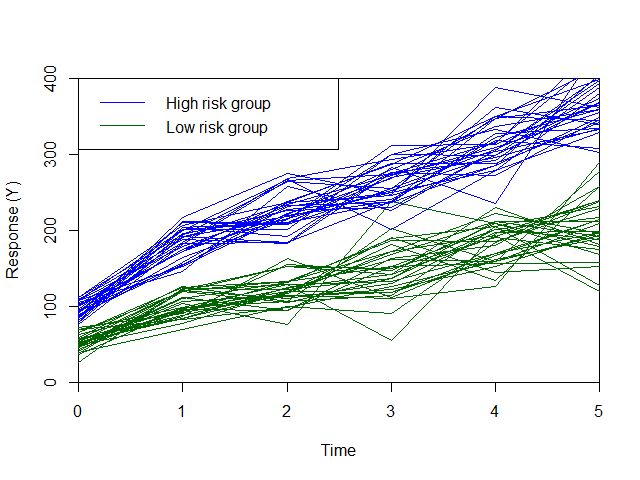
\includegraphics[scale=0.5]{mainmatter/chapter_3_blmm/random_slope_dummy_data.png}
	\caption{Individual profiles of 30 subjects from each group.}
	\label{fig : random_slope_dummy_data}
\end{figure}

In a LMM is quite common to use histogram of Empirical Bayes estimates of random effects to detect groups of individuals. However \citet{verbeke_linear_1996} have shown that if the prior is misspecified(for e.g. if in our example we use a univariate normal distribution), then the histogram of estimates of random effects will be shrunk towards the prior distribution. Thus it would be impossible to classify the subjects into different categories based on empirical bayes estimates of random effects as they are incorrect. A solution to this problem is using a mixture of Gaussian components for random effects distribution. Such a linear mixed model is termed as a Heterogeneity model.

\subsection{Bayesian heterogeneity model}
\label{subsec : bhtge}
The formal definition of a Bayesian heterogeneity model can be given by extending the Bayesian linear mixed model definition given in section \ref{sec : blmm}. Since, now the random effects have a Gaussian mixture distribution we will use the following notation to express the distribution mathematically.

$$\boldsymbol{b}_i \sim \sum_{k=1}^{K} \eta_k N_q(\boldsymbol{b}_k^C, G_k)$$\\
where $\boldsymbol{b}_k^C$ and $G_k$ are the mean vector and covariance matrices for the $k^\text{th}$ component in the mixture distribution respectively. The vector $\boldsymbol{\eta} = (\eta_1, \eta_2, \ldots, \eta_K)$ is the weight distribution for the component densities. The vector $\boldsymbol{S}=(S_1, S_2, ..., S_n)$ represents the allocation vector for the $n$ subjects. Since we are following the Bayesian paradigm, in addition to prior distribution for $\boldsymbol{\beta}$ and $\sigma^2$ we also have prior for $\boldsymbol{\nu} = (\boldsymbol{b}_1^C, \boldsymbol{b}_2^C, \ldots, \boldsymbol{b}_K^C, G_1, G_2, \ldots, G_K, \boldsymbol{\eta})$.


\section{Estimation of parameters in the Bayesian heterogeneity model}
In this section we will discuss some of the challenges in Bayesian estimation of parameters in the Bayesian heterogeneity model. We will also discuss the approaches we used to deal with them in this thesis.

\subsection{Marginal vs. Hierarchical model}
Suppose that in our heterogeneity model we know the alloations $S_i$ for each subject. Then conditional on knowing $S_i=k$ the following LMM equation has a hierarchical interpretation.

\begin{equation}
\begin{split}
\boldsymbol{y}_i|\boldsymbol{b}_{i}, S_i &\sim N(\boldsymbol{X}_{i}\boldsymbol{\beta} + \boldsymbol{Z}_{i}\boldsymbol{b}_{i},\boldsymbol{\varepsilon}_{i})\\ 
\boldsymbol{\varepsilon}_{i} &\sim N_{m_i}(\boldsymbol{0}, R_i)
\end{split}
\end{equation}

One can however integrate out the random effects $\boldsymbol{b}_{i}$ and obtain the corresponding marginal Bayesian heterogeneity model,

\begin{equation}
\begin{split}
\boldsymbol{y}_i|S_i &\sim N(\boldsymbol{X}_{i}\boldsymbol{\beta} + \boldsymbol{Z}_{i}\boldsymbol{b}_k^C, \boldsymbol{\varepsilon}_{i}^*)\\ 
\boldsymbol{\varepsilon}_{i}^* &\sim N_{m_i}(\boldsymbol{0}, \boldsymbol{Z}_{i}G_k\boldsymbol{Z}_{i}^T+ R_i)
\end{split}
\end{equation}

The marginal model is recommended by \citet{fruhwirth-schnatter_bayesian_2004} for good mixing of chains, and while doing the simulation study(presented in chapter \ref{ch : simulation_study}) we found that claim to be true. However, the marginal model took quite a long time for each iteration. It also did not give posterior estimates of the random effects $\boldsymbol{b}_i$ which were required for calculation of certain definitions of DIC (discussed in chapter \ref{ch : model_selection}). Besides we found that a model with hierarchical centering took less time for each iteration and had as much autocorrelation in the posterior density samples as with the use of the marginal model.

\subsection{Hierarchical centering}
The random effects $\boldsymbol{b}_i$ in a mixed model could be seen as random deviations from the fixed effects $(\boldsymbol{\beta})$ with a mean $\boldsymbol{0}$. For a longitudinal data set, it means that the overall effect of a covariate such as the intercept for a subject should be the sum of both fixed and random effects. In this case matrices $\boldsymbol{X}$ and $\boldsymbol{Z}$ both share columns corresponding to the variable intercept. To enforce the mean $\boldsymbol{0}$ on the random effects in a mixture distribution of random effects, the following condition should be satisfied.

\begin{equation}
\label{eq : non_centred_constraint}
E(\boldsymbol{b}_i | \boldsymbol{\nu}) = \sum_{k=1}^{K} \eta_k N_q(\boldsymbol{b}_k^C, G_k) = 0
\end{equation}

where $\boldsymbol{\nu}$ is defined in section \ref{subsec : bhtge}. This further means that $E(\boldsymbol{y}_i | \boldsymbol{\nu}) = \boldsymbol{X}_{i}\boldsymbol{\beta}$. This parametrization, which was also used in the original paper on Heterogeneity model \citep{verbeke_linear_1996} is called the noncentralized parametrization. The centralized parametrization assumes that the random effects are not deviations from the fixed effects and are centred around a non zero mean.\\

The choice of parametrization has an effect on the rate of convergence of the chains in MCMC process. While doing the simulation study we observed that imposing the constraint in equation \ref{eq : non_centred_constraint} drastically slowed the convergence as well increased the autocorrelation in parameter estimates. Thus, in this thesis we have only used hierarchically centred parametrization.

\subsection{Starting values}

\subsection{Choice of priors}
\label{subsec : choice_priors}
Since we are following a Bayesian paradigm, parameters in the Bayesian heterogeneity model are random variables and thus need to have a prior distribution. There are certain difficulties in specifying the prior though, especially that it can be difficult to implement theoretically preferred prior distributions. As an example we will begin with the choice of prior for the mean $(b_k^C)$ and covariance matrix $(G_k)$ of component densities in the mixture distribution of random effects. Both $b_k^C$ and $G_k$ are unknown, and hence to obtain the joint posterior as a known density one is forced to specify the conditionally conjugate prior $b_k^C | G_k \sim N(\boldsymbol{\mu}_0, \frac {G_K} {N_0})$ and $G_k^{-1} \sim \mathcal{W} (n_0, \Psi)$. Here $\boldsymbol{\mu}_0, N_0, n_0, \Psi$ are the hyperparameters for the corresponding prior distributions. Since JAGS only allows specifying marginal priors, one will have to specify a multivariate T distribution for $b_k^C$. However the problem with this approach is that the choice of the right hyperparameters is debatable \citep[pg. 192]{fruhwirth-schnatter_finite_2013} and even if one does, the extra computationally intensive procedure does not provide much advantage in practice. It is thus a widespread practice to use independent priors for the mean $(b_k^C)$ and covariance matrix $(G_k)$ \citep[chap. 17]{gelman_data_2006}. For e.g. a common non informative prior for $b_k^C$ (say, having only random intercept and slope) is $N(\boldsymbol{0}, \begin{bmatrix}10^5 & 0 \\ 0 & 10^5\end{bmatrix})$. This prior is equivalent to specifying indepedent diffuse univariate normal priors for the mean of random intercept and for the mean of random slope.

\subsubsection{Choice of prior for covariance matrix}
The choice of prior for the covariance matrix $(G_k)$ is an interesting problem. \citet[pg. 260]{lesaffre_bayesian_2012} suggest using an inverse wishart prior with small diagonal elements for the scale hyperparameter and degrees of freedom hyperparameter equal to the dimension of $G_k$. For e.g $IW(\begin{bmatrix}0.01 & 0 \\ 0 & 0.01\end{bmatrix}, 2)$ could be one such prior. For precision matrix $G_k^{-1}$ one can use the wishart prior $W(\begin{bmatrix}10 & 0 \\ 0 & 10\end{bmatrix}, 2)$. i.e. the scale of wishart prior is inverse of the scale hyperparameter for inverse wishart distribution. As we found later in our simulations, a big value for diagnoal elements of scale matrix of wishart distribution influenced the posterior more than the likelihood did.\\

 \citet[pg. 260]{lesaffre_bayesian_2012} also suggest using indepdent gamma priors for random intercept and random slope and uniform prior $U(-1,1)$ for the correlation between the two. The upside of this approach is that it gives almost the same estimates as one can get from frequentist analysis, but the downside is that MCMC iterations are slower because the posterior is not available as a known density. Another benefit of this approach, as we later found out during simulations is that when the mixture distribution is overfitted, then the extra components tend to have very high variance estimates for random intercept and random slope. This property can be used to make decisive posterior predictive checks.

\subsubsection{Choice of priors for $\boldsymbol{\beta}$ and $\sigma^2$}
We assume that the parameters $\boldsymbol{\beta}$ and $\sigma^2$ are indepdent from $\boldsymbol{b}_1^C, \boldsymbol{b}_2^C, ..., \boldsymbol{b}_K^C, G_1, G_2, ..., G_K, \boldsymbol{\eta}$. The problem of choosing a conjugate prior for $\boldsymbol{\beta}$ and $\sigma^2$ is similar to what we discussed in the section above. The solution thus is alike, i.e. using indepdent univariate normal priors such as $N(0, 10000)$ for each of the $\beta_d$ and a $\text{Gamma}(0.0001, 0.0001)$ prior for $\tau = \frac 1 {\sigma^2}$ \citep[chap. 17]{gelman_data_2006}.

\subsubsection{Choice of prior for $\boldsymbol{\eta}$}
The conjugate prior for the weight distribution $\boldsymbol{\eta}$ is the Dirichlet prior $\text{Dir}(a_0, a_1,..., a_K)$. \citet[pg. 105]{fruhwirth-schnatter_finite_2013} suggest choosing values of hyperparameters $a_0, a_1,..., a_K$ to be greater than 1 in cases where one of the components is nearly empty. If one chooses the hyperparameters to be equal to 1 then label switching is observed whenever one of the components is nearly empty. We found out during the simulation study that choosing larger values for the hyperparameter indeed mitigated the issue of label switching, however it did also gave parameter estimates far from the real ones. 

\subsection{Label Switching}
\label{subsec : label_switching_blmm}
We use a mixture distribution for random effects in the Bayesian heterogeneity model. However we do not know the allocation vector $\boldsymbol{S}$ in advance. In this case the mixture likelihood for the response $\boldsymbol{y}$ is given by the equation \ref{eq : obs_data_likelihood}. The mixture likelihood function is symmetrical and has $K!$ modes \citep[pg. 44]{fruhwirth-schnatter_finite_2013}. This creates a problem called label switching while doing the MCMC procedure.\\

The label switching problem can be explained with the following example. Suppose we have a mixture distribution $0.5N(5,1) + 0.5N(7,1)$ of two components $C_1$ and $C_2$ and we have few observations sampled from the mixture. Using the MCMC procedure we can one estimate the parameters of the two components. The MCMC procedure for missing data models like mixture models uses a technique called data augmentation. The idea of data augmentation is similar to the frequentist EM algorithm. ie. we begin with some random allocation vector $\boldsymbol{S}_\text{initial}$ and estimate parameters using the complete data likelihood. An example expression of a complete data likelihood for Bayesian heterogeneity model is expression \ref{eq : complete_data_likelihood}. For the MCMC sampler, labels $\mu_1$ and $\mu_2$ exist for the two means, however either one can correspond to $\mu_{C1}$ or $\mu_{C2}$. i.e. Labels are not associated with actual components from the beginning. Assume that the allocation vector $\boldsymbol{S}_\text{initial}$ is such that it assigns all observations from component $C_1$ under label 1 and all observations from component $C_2$ under label 2. Under such a scheme a posterior sample $(\mu_1,\mu_2) = (5,7)$ is likely. However if we take a conjugate of this allocation vector then $(\mu_1,\mu_2) = (7,5)$ is also likely to be sampled. This can be attributed to the fact that we have a mixture likelihood function which is bimodal.\\

Now let us imagine a scenario where because of a certain $\boldsymbol{S}_\text{initial}$, the sampled parameter estimates are $(\mu_1, \mu_2) = (5.5,6.5)$. So far it seems $\mu_1$ represents $\mu_{C1}$ and $\mu_2$ represents $\mu_{C2}$. Now in the next step the Gibbs sampler will estimate the allocation vector $\boldsymbol{S}$ conditional on these estimates. Suppose that in this step an observation with value 6.5 which was originally from component $C_2$, gets allocated to component $C_1$ and similarly an observation with value 5.5 from component $C_1$ gets allocated to $C_2$. Unless we impose some constraint like $\mu_1 < \mu_2$, under the current scenario even $(\mu_1,\mu_2) = (6.5, 5.5)$ is likely to be be sampled by MCMC. If the sampler keeps on arbitrarily switching between the two equivalent posterior regions, then because of this label switching, one may obtain a bimodal posterior for both $\mu_1$ and $\mu_2$. Thus both posteriors may well remain partially explored and thus any inference based on these posteriors will not be useful.

\subsubsection{Dealing with label switching}
One of the techniques we used for dealing with label switching was imposing an identifiability constraint such as $\mu_1 < \mu_2$. The difficulty with this approach is that it is easier to do in univariate mixtures but not with multivariate mixtures. For e.g. a multivariate mixture that we have is mixture distribution for the joint distribution of random intercept and random slope. In this thesis the multivariate case was handled by putting an identifiability constraint only on either the random intercept or the random slope depending upon the variance of each random effect. It is interesting to note that if more components than needed were chosen, then label swtiching is unavoidable, and should also be seen as an indicator for overfitting \citep[pg. 104]{fruhwirth-schnatter_finite_2013}.\\

One of the other interesting techniques to deal with label switching is postprocessing of MCMC chains by relabeling the output\citep{richardson_bayesian_1997,stephens_dealing_2000}. We too employed this technique in the approximation of marginal likelihood (section \ref{sec : marginal_likelihood}), as that procedure also involves running further MCMC chains (expression \ref{eq : rao_blackwellization_wishart}). As we later figured out in our simulations, without careful relabeling of output one may obtain a Bayes factor $\to 0$ and thus reject the model outright.